\documentclass{beamer}
\usetheme{CambridgeUS}

\usepackage{tikz,pgfplots}
\usepackage{amsmath,amssymb}
\usepackage{xcolor}
\usepackage{graphicx}
\usepackage{wasysym}
\usepackage[language=english, backend=biber, style=alphabetic, sorting=nyt]{biblatex}

\addbibresource{bibliography.bib}

\title{SIKE - PQC based on isogenies}
\author{Simon Pohmann}
\institute{University of Passau}

\newcommand{\R}{\mathbb{R}}
\newcommand{\F}{\mathbb{F}}
\newcommand{\Z}{\mathbb{Z}}
\renewcommand{\O}{\mathcal{O}}

\newtheorem{prob}{Problem}

\pgfplotsset{compat=1.16}
\pgfplotsset{every x tick label/.append style={font=\tiny}}
\pgfplotsset{every y tick label/.append style={font=\tiny}}

\begin{document}

\frame{\titlepage}

\frame{
    \frametitle{Contents}
    \tableofcontents
}

\section{Elliptic Curves}

\begin{frame}
\frametitle{Elliptic Curves}
Let $K$ be a field of characteristic $\neq 2, 3$.
\begin{definition}
    A (possibly non-smooth) \emph{elliptic curve} $E$ is the zero set
    \begin{equation*}
        \{ (x, y) \ | \ F(x, y) = 0 \} \subseteq \bar{K}^2
    \end{equation*}
    of some irreducible polynomial $F(x, y) = y^2 - x^3 - Ax - B \in K[x, y]$ together with a point $\O = \infty$ at infinity.
\end{definition}
\pause
\begin{definition}
    An elliptic curve $E: y^2 = x^3 + Ax + B$ is called smooth, if the \emph{discriminant}
    \begin{equation*}
        \Delta(E) := -16(27 B^2 + 4 A^3) \neq 0
    \end{equation*}
\end{definition}
\end{frame}

\begin{frame}
\frametitle{Examples}
\begin{columns}
    \begin{column}{0.49\textwidth}
        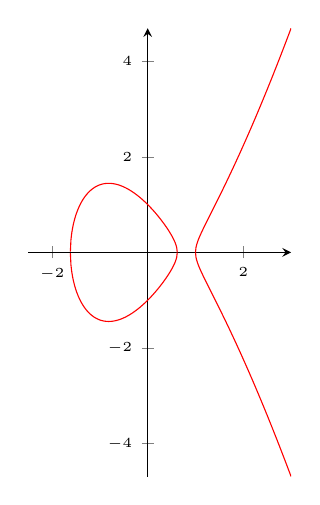
\begin{tikzpicture}
            \begin{axis}[
                axis lines = middle,
                xmin = -2.5,
                axis equal image = true,
                samples = 200
            ]
                \addplot[red, domain=1:3] {sqrt(\x*\x*\x - 2*\x + 1)};
                \addplot[red, domain=1:3] {-sqrt(\x*\x*\x - 2*\x + 1)};
                \addplot[red, domain=-1.618:0.618] {sqrt(\x*\x*\x - 2*\x + 1)};
                \addplot[red, domain=-1.618:0.618] {-sqrt(\x*\x*\x - 2*\x + 1)};
            \end{axis}
        \end{tikzpicture}

        points of $E: y^2 = x^3 - 2x + 1$ in $\R^2$
    \end{column}
    \begin{column}{0.49\textwidth}
        \pause
        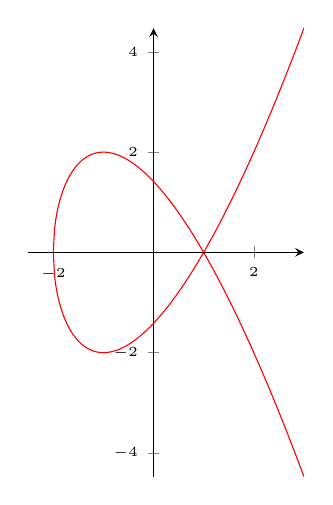
\begin{tikzpicture}
            \begin{axis}[
                axis lines = middle,
                xmin = -2.5,
                axis equal image = true,
                samples = 200
            ]
                \addplot[red, domain=-2:3] {sqrt(\x*\x*\x - 3*\x + 2)};
                \addplot[red, domain=-2:3] {-sqrt(\x*\x*\x - 3*\x + 2)};
            \end{axis}
        \end{tikzpicture}

        points of $E: y^2 = x^3 - 3x + 2$ in $\R^2$
    \end{column}
\end{columns}
\end{frame}

\section{Isogenies}

\subsection{Morphisms}

\begin{frame}
    \frametitle{Coordinate ring}
    \begin{definition}
        Let $E: y^2 = x^3 + Ax + B$ be an elliptic curve. Then 
        \begin{equation*}
            K[E] := K[x, y] / (F), \quad F(x, y) = y^2 - x^3 - A x - B
        \end{equation*}
        is the \emph{coordinate ring} of $E$.
    \end{definition}
    \pause
    \begin{center}
        $f \in K[E]$ are the ``polynomial functions'' defined on $E$
    \end{center}
    \pause
    \begin{definition}
        Let $E: y^2 = x^3 + Ax + B$ be an elliptic curve. Then define the function field $K(E)$ as the quotient field of $K[E]$.
    \end{definition}
\end{frame}

\begin{frame}
    \frametitle{Rational functions - Example}
    Consider $E: y^2 = x^3 - x + 1$ and $f = \frac {(y - 1)(x + 1)} {x(x + 1)} \in K(E)$.

    \vspace{2ex}
    We want to evaluate $f$.
    \pause
    \begin{itemize}
        \item at $(1, 1) \pause \quad \Rightarrow \quad f(1, 1) = 0$
        \pause
        \item at $(-1, -1) \pause \quad \Rightarrow \quad f(1, 1) = 2$
        \pause
        \item at $(0, 1) \pause \quad \Rightarrow \quad f(0, 1) = -\frac 1 2$
    \end{itemize}
    \pause
    \vspace{2ex}
    However: $\frac 1 x \in K(E)$ cannot be defined at $(0, 1)$.
\end{frame}

\begin{frame}
    \frametitle{Morphisms}
    Now we consider maps $E \to E'$ for elliptic curves $E, E'$.
    \begin{equation*}
        \phi: E \to E', \quad (x, y) \mapsto (f(x, y), \ g(x, y)) \quad \text{for} \ f, g \in \bar{K}(E)
    \end{equation*}
    \pause
    These are called \emph{morphisms}.
    \pause
    \vspace{2ex}
    \begin{itemize}
        \item $f(x, y), g(x, y)$ must satisfy the equation of $E'$ for all $(x, y) \in E$
        \\$\Rightarrow \ f, g$ satisfy the equation of $E'$ in $K(E)$ (Hilbert's Nullstellensatz)
        \pause
        \item Define $\O := (\frac {\neq 0} 0, *) = (*, \frac {\neq 0} 0) = (\frac {\neq 0} 0, \frac {\neq 0} 0)$
        \\$\Rightarrow$ one can always define $f(x, y), \ g(x, y) \in E'$
        \pause
        \item If $f, g \in K(E)$ say $\phi$ is defined over $K$
        \pause
        \item What about $\phi(\O)$?
    \end{itemize}
\end{frame}

\subsection{Isogenies}

\begin{frame}
    \frametitle{Isogenies}
    Let $E, E'$ be elliptic curves.
    \begin{definition}
        A morphism $E \to E'$ that maps $\O$ to $\O$ is called \emph{isogeny}.
    \end{definition}
    \pause
    \begin{definition}
        A bijective isogeny $E \to E'$ whose inverse is an isogeny is called \emph{isomorphism}.
    \end{definition}
\end{frame}

\begin{frame}
    \frametitle{Isogenies - Example}
    Let $E: y^2 = x^3 - x + 1$ and $E': y^2 = x^3 - 4x + 8$.
    \pause
    \begin{equation*}
        \phi: E \to E', \quad \O \mapsto \O, \ (x, y) \mapsto (2x, \sqrt{8}y)
    \end{equation*}
    \pause
    Have
    \begin{equation*}
       (\sqrt{8}y)^2 = (2x)^3 - 4(2x) + 8 \ \text{in} \ K[E]
    \end{equation*}
    \pause
    So $\phi$ is a well-defined isogeny.

    \pause
    Its inverse is
    \begin{equation*}
        \phi^{-1}: E' \to E, \quad \O \mapsto \O, \ (x, y) \mapsto (\frac 1 2 x, \frac 1 {\sqrt{8}} y)
    \end{equation*}
    \pause
    So $\phi$ is an isomorphism.
\end{frame}

\subsection{Isomorphisms}

\begin{frame}
    \frametitle{j-invariant}
    Let $E: y^2 = x^3 - x + 1$ and $E': y^2 = x^3 - 4x + 8$. Then
    \begin{equation*}
        \phi: E \to E', \quad \O \mapsto \O, \ (x, y) \mapsto (2x, \sqrt{8}y)
    \end{equation*}
    is an isomorphism.
    \pause

    Recall the discriminant
    \begin{equation*}
        \Delta(E) := -16(27 B^2 + 4 A^3) \neq 0
    \end{equation*}
    \pause
    \begin{definition}
        The \emph{j-invariant} is
        \begin{equation*}
            j(E) := \frac {(-48A)^3} {\Delta(E)}
        \end{equation*}
    \end{definition}
    \pause
    \begin{equation*}
        j(E) = \frac {110592} {-368} = \frac {6912} {23}, \quad j(E') = \frac {7077888} {-23552} = \frac {6912} {23}
    \end{equation*}
\end{frame}

\begin{frame}
    \frametitle{j-invariant}
    \begin{definition}
        The \emph{j-invariant} is
        \begin{equation*}
            j(E) := \frac {(-48A)^3} {\Delta(E)} = \frac {(-48A)^3} {-16(27B^2 + 4A^3)}
        \end{equation*}
    \end{definition}
    \begin{theorem}
        $E \cong E'$ if and only if $j(E) = j(E')$
    \end{theorem}
\end{frame}

\section{The Group Structure}

\begin{frame}
    \frametitle{Geometric Group Structure}

    \begin{columns}
        \begin{column}{0.49\textwidth}
            \begin{tikzpicture}
                \begin{axis}[
                    axis lines = middle,
                    axis equal image = true,
                    xmax = 3.5,
                    xmin = -3.2,
                    samples = 200
                ]
                    \addplot[red, domain=1:3] {sqrt(\x*\x*\x - 2*\x + 1)};
                    \addplot[red, domain=1:3] {-sqrt(\x*\x*\x - 2*\x + 1)};
                    \addplot[red, domain=-1.618:0.618] {sqrt(\x*\x*\x - 2*\x + 1)};
                    \addplot[red, domain=-1.618:0.618] {-sqrt(\x*\x*\x - 2*\x + 1)};

                    \only<2->{
                        \node[blue, label={120:{$P$}}, circle, fill, inner sep = 1pt] at (axis cs: 0, 1) {};
                        \node[blue, label={120:{$Q$}}, circle, fill, inner sep = 1pt] at (axis cs: -1.618, 0) {};
                    }
                    \only<3->{
                        \addplot[blue, domain=-3.2:3] {0.618*\x + 1};
                    }
                    \only<4->{
                        \node[blue, label={120:{$R$}}, circle, fill, inner sep = 1pt] at (axis cs: 2, 2.236) {};
                    }
                    \only<5->{
                        \node[blue, label={$P + Q$}, circle, fill, inner sep = 1pt] at (axis cs: 2, -2.236) {};
                    }
                \end{axis}
            \end{tikzpicture}
        \end{column}
        \begin{column}{0.49\textwidth}
            \begin{theorem}
                Each line meets $E$ in exactly three points (with multiplicity)
            \end{theorem}
            \pause
            Define $P +_{\mathrm{geo}} Q$ by
            \pause
            \begin{itemize}
                \item $L :=$ line through $P, Q$
                \begin{itemize}
                    \item If $P = Q$ use tangent
                \end{itemize}
                \pause
                \item $R :=$ third intersection point of $L$ and $E$
                \pause
                \item $P +_{\mathrm{geo}} Q := -R$
                \begin{itemize}
                    \item $-(x, y) := (x, -y)$
                \end{itemize}
            \end{itemize}
            \vspace{3ex}
            \pause
            Set $\O +_{\mathrm{geo}} P = P +_{\mathrm{geo}} \O = P$.
        \end{column}
    \end{columns}
\end{frame}

\begin{frame}
    \frametitle{Algebraic Group Structure}
    From Cryptanalysis we know:
    \begin{theorem}
        The coordinate ring $K[E]$ is a Dedekind domain.
    \end{theorem}
    \pause
    \begin{theorem}
        There is a bijection
        \begin{equation*}
            \rho: E \to \mathrm{Cl}(\bar{K}[E]), \quad \O \mapsto \overline{\bar{K}[E]}, \ (\lambda, \mu) \mapsto \overline{\langle x - \lambda, y - \mu \rangle}
        \end{equation*}
        where $\mathrm{Cl}(\bar{K}[E])$ is the ideal class group of $\bar{K}[E]$.
    \end{theorem}
    \pause
    \begin{definition}
        Define $+_{\mathrm{alg}}$ on $E$ by $P +_{\mathrm{alg}} Q = \rho^{-1}(\rho P \cdot \rho Q)$.
    \end{definition}
\end{frame}

\begin{frame}
    \frametitle{Rational Group Structure}
    Let $E: y^2 = x^3 + Ax + B$.
    \pause
    For $P = (x_1, y_1), \ Q = (x_2, y_2) \neq -P$ define
    \begin{align*}
        \lambda &:= \begin{cases}
            \frac {y_2 - y_1} {x_2 - x_1} & \text{if} \ x_1 \neq x_2 \\
            \frac {3x_1^2 + A} {2 y_1} & \text{otherwise}
        \end{cases} \\
        \uncover<3->{
            x_3 &:= -x_1 - x_2 + \lambda^2 \\
        }
        \uncover<4->{
            y_3 &:= -y_1 + \lambda(x_1 - x_3) \\
        }
        \uncover<5->{
            P +_{\mathrm{poly}} Q &:= (x_3, y_3)
        }
    \end{align*}
    \pause
    \pause
    \pause
    \pause
    Further $P +_{\mathrm{poly}} (-P) := \O$.
\end{frame}

\begin{frame}
    \frametitle{Elliptic Curves as Groups}

    \pause
    \begin{theorem}
        Let $E$ be an elliptic curve. Then $+ := +_{\mathrm{geo}} = +_{\mathrm{alg}} = +_{\mathrm{poly}}$.
    \end{theorem}

    \pause
    \begin{corollary}
        Let $E$ be an elliptic curve. Then
        \pause
        \begin{itemize}
            \item $E$ with $+$ is a group
            \pause
            \item $E$ is abelian
            \pause
            \item $E$ has neutral element $\O$
        \end{itemize}
    \end{corollary}
    \pause
    For fields $\bar{K} | L | K$ let $E(L) := E \cap L^2 \cup \{ \O \}$ be the $L$-rational points.
    \pause
    \begin{corollary}
        $E(L)$ is a subgroup of $E$
    \end{corollary}
\end{frame}

\subsection{Isogenies and the group structure}

\begin{frame}
    \frametitle{Isogenies}

    Let $E, E'$ be elliptic curves. \cite{arithmetic_elliptic_curves} shows
    \pause
    \begin{theorem}
        An isogeny $\phi: E \to E'$ is a group homomorphism with finite kernel.
    \end{theorem}

    \pause
    \begin{theorem}
        Let $\Phi \leq E$ be a finite subgroup. Then there is a unique elliptic curve $\tilde{E}$ and a (separable) isogeny $\phi: E \to \tilde{E}$ with $\ker \phi = \Phi$ (up to isomorphism).
    \end{theorem}
    \begin{center}
        Write $E/\Phi = \tilde{E}$
    \end{center}

    \pause
    \begin{prob}[Isogeny Path]
        Given elliptic curves $E, E'$ defined over $\F_q$ with $\#E(\F_q) = \#E'(\F_q)$, find an isogeny $E \to E'$ of smooth degree ($\mathrm{deg}\phi := \#\ker\phi$).
    \end{prob}
    \begin{center}
        smooth $\sim$ only small factors
    \end{center}
\end{frame}

\section{SIDH}

\begin{frame}
    \frametitle{Idea}
    \begin{center}
        \includegraphics{scheme1.pdf}

        \pause
        How to compute $E/\langle A, B \rangle$?
    \end{center}
\end{frame}

\begin{frame}
    \frametitle{Supersingular Curves}
    \begin{definition}
        Define $\mathrm{End}(E) := \{ \phi: E \to E \ | \ \phi \ \text{isogeny} \}$, equipped with addition $+$ and composition $\circ$.
    \end{definition}
    \pause
    \begin{definition}
        Assume $\mathrm{char}(K) \neq 0$. Then $E$ is called supersingular, if $\mathrm{End}(K)$ is not commutative.
    \end{definition}
    \pause
    \begin{theorem}
        Let $E$ be supersingular, defined over $\F_{p^2}$. If $j(E) \neq 0, 1728$ then 
        \begin{equation*}
            E\left( \F_{p^2} \right) \cong \left( \Z / (p \pm 1)\Z \right)^2
        \end{equation*}
    \end{theorem}
    \pause
    We also need $E[n] := \left\{ P \in E\left(\F_{p^2}\right) \ \middle| \ \mathrm{ord}P \ | \ n \right\} \leq E\left(\F_{p^2}\right)$
\end{frame}

\begin{frame}
    \frametitle{Supersingular Isogeny Diffie-Hellman}

    \begin{theorem}
        Let $E$ be supersingular, defined over $\F_{p^2}$. If $j(E) \neq 0, 1728$ then 
        \begin{equation*}
            E\left( \F_{p^2} \right) \cong \left( \Z / (p \pm 1)\Z \right)^2
        \end{equation*}
    \end{theorem}
    \begin{center}
        \uncover<2->{
            \only<1-2|handout:0>{\includegraphics{scheme2_0.pdf}}
            \only<3|handout:0>{\includegraphics{scheme2_1.pdf}}
            \only<4|handout:0>{\includegraphics{scheme2_2.pdf}}
            \only<5|handout:0>{\includegraphics{scheme2_3.pdf}}
            \only<6|handout:0>{\includegraphics{scheme2_4.pdf}}
            \only<7|handout:0>{\includegraphics{scheme2_5.pdf}}
            \only<8->{\includegraphics{scheme2_6.pdf}}
        }
    \end{center}
    \pause
    \pause
    \pause
    \pause
    \pause
    \pause
    \pause
    \pause
    \begin{equation*}
        \text{Claim:} \ E / \langle A, B \rangle \cong E / \langle B \rangle / \langle A' \rangle
    \end{equation*}
\end{frame}

\begin{frame}
    \frametitle{Computing Isogenies}

    \pause
    \begin{itemize}
        \item $E, P_A, Q_A, P_B, Q_B$ are fixed, namely $E: y^2 = x^3 + 6x^2 + x$
        \pause
        \item $nP$ using ``double-and-add''
        \pause
        \item So its left to compute $E / \langle A \rangle$ and $E \to E/\langle A \rangle$
    \end{itemize}
    \pause

    \begin{theorem}[Vélu's formulas]
        Let $G \leq E$ be finite and $\phi: E \to E/G$. With $G' = G \setminus \{0\}$ have
        \pause
        \begin{itemize}
            \item $E/G: y^2 = x^3 + A'x + B'$ where
            \pause
            \begin{align*}
                A' := A - 5\sum_{(x, y) \in G'} 3x^2 + A, \quad
                B' := B - 7\sum_{(x, y) \in G'} 5x^3 + 3Ax + B
            \end{align*}
            \pause
            \item For $P \not\in G$, $\phi(P)$ is
            \begin{align*}
                \left( x(P) + \sum_{Q \in G'} x(P + Q) - x(Q), \quad y(P) + \sum_{Q \in G'} y(P + Q) - y(Q) \right)
            \end{align*}
        \end{itemize}
    \end{theorem}
\end{frame}

\begin{frame}
    \frametitle{Computing Isogenies}
    \begin{theorem}[Vélu's formulas]
        Let $G \leq E$ be finite and $\phi: E \to E/G$. With $G' = G \setminus \{0\}$ have
        \begin{itemize}
            \item $E/G: y^2 = x^3 + A'x + B'$ where
            \begin{align*}
                A' := A - 5\sum_{(x, y) \in G'} 3x^2 + A, \quad
                B' := B - 7\sum_{(x, y) \in G'} 5x^3 + 3Ax + B
            \end{align*}
            \item For $P \not\in G$, $\phi(P)$ is
            \begin{align*}
                \left( x(P) + \sum_{Q \in G'} x(P + Q) - x(Q), \quad y(P) + \sum_{Q \in G'} y(P + Q) - y(Q) \right)
            \end{align*}
        \end{itemize}
    \end{theorem}

    \pause
    However, $\#G = 2^{e_A}$ resp. $\#G = 3^{e_B}$ is exponential
    \pause
    \\$\Rightarrow$ Decompose $\phi = \phi_1 \circ ... \circ \phi_e$ where $\#\ker\phi_i = 2$ resp. $3$
\end{frame}

\subsection{Isogeny Paths}

\begin{frame}
    \frametitle{Isogeny Path}
    Decompose $\phi = \phi_1 \circ ... \circ \phi_e$ where $\ker\phi_i = 2$ resp. $3$
    \begin{prob}[Isogeny Path]
        Given elliptic curves $E, E'$ defined over $\F_q$ with $\#E(\F_q) = \#E'(\F_q)$, find an isogeny $E \to E'$ of smooth degree ($\mathrm{deg}\phi := \#\ker\phi$).
    \end{prob}
    
    \begin{columns}
        \begin{column}{0.4\textwidth}
            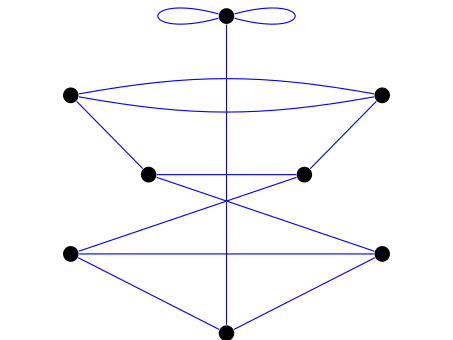
\includegraphics[width = \textwidth]{isogeny_graph1.pdf}
        \end{column}
        \begin{column}{0.4\textwidth}
            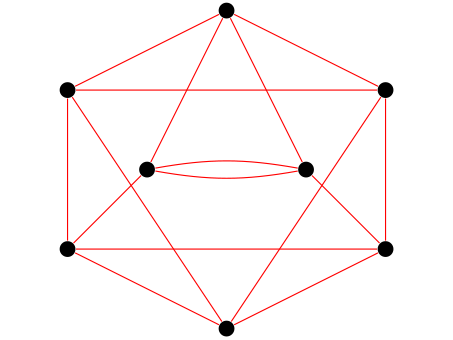
\includegraphics[width = \textwidth]{isogeny_graph2.pdf}
        \end{column}
        \begin{column}{0.2\textwidth}
            nodes $\sim$ j-invariants
            
            \vspace{3ex}

            edges $\sim$ isogenies
        \end{column}
    \end{columns}
    \begin{center}
        2 resp. 3-isogeny graph of $\F_{97^2}$ from \cite{mathematics_isogeny_crypto}
    \end{center}
\end{frame}

\begin{frame}
    \frametitle{References}
    \printbibliography

    \begin{center}
        Thank you for your attention!
    \end{center}
\end{frame}
\end{document}